\documentclass{article}
\usepackage{hyperref}
\usepackage{graphicx}
\title{acm.mst.edu Design Documentation}
\author{Kevin Schoonover}
\date{\today}

\begin{document}

\maketitle

\tableofcontents

\section{Introduction}
\subsection{Purpose}
In order to start on a large-scale project like the ACM-General website, I
believe that it is important to first talk about why we are doing the project.

The main reason that that I started this process originally was threefold.
Firstly, the majority of the System Administrator job was updating
the old ACM-General website by manually uploading photos and inputting them into
a WordPress site and then creating WordPress events; I personally believed that we
could create a more personalized and intelligent approach which would allow these
repetitive tasks to be more easily automated. Secondly, I wanted to create a
more succinct and refined user experience for everyone who interacted with the
website thereby increasing user productivity and activity within ACM.
Lastly, I believed that the website was capable of so much more than a
'attractive' flier and an event share. Features like automatically managing SIGs,
allowing for developer interaction through an API, and much more would allow
for ACM to grow in a more extensive and intelligent way. All of this and
more will be discussed throughout this Design documentation.

\subsection{Tools / Prerequisite Knowledge}
Some tools, frameworks, and languages one should attempt to familiarize
themselves with to jump head-first into the project:
\begin{itemize}
    \item Django (\url{https://docs.djangoproject.com/en/1.11/}) - Web
          Framework and back-end which runs all of the webpage interaction.
    \item Django REST Framework (\url{http://www.django-rest-framework.org/}) -
          A nice library which helps to automatically configure and manage the
          API.
    \item Git (\url{http://www.sphinx-doc.org/en/stable/}) - Source control
          management software which allows for intelligent sharing and
          management of code.
    \item Jenkins (\url{https://jenkins.io/}) - Another continuous
          integration platform which automatically deploys the website.
    \item Python3 (\url{https://docs.python.org/3/}) - The main programing
          language used in essentially everything we write.
    \item Sphinx (\url{http://www.sphinx-doc.org/en/stable/}) - Automatic
          documentation suite which is a python standard.
    \item Stripe (\url{https://stripe.com/}) - Payment gateway in which all of
          the payments will run through.
    \item Travis CI (\url{https://travis-ci.org/}) - Continuous integration
          platform which runs the automated testing of the code base.
\end{itemize}

\section{Design}
\subsection{Web API}
In order to improve overall modularity and extensibility, a RESTful Web API
exposing the majority, if not all, of the Django models must be implemented.

\subsubsection{Schema}
The URL scheme for the web-api will be as follows:
\\ \texttt{/web-api/<api\_version>/<model\_name>/(model\_pk)}
\\
\\
\textbf{api\_version} (Required): Whatever version of the API that is used. All
previous versions of the API will be reserved (unless expressly deprecated to
all users of the API) in order to preserve backwards compatibility of software
which may be legacy. The most current version will be named \texttt{latest}.
% Full Indent
\\
\textbf{model\_name} (Required): The name of the model which the user is
attempting to access with the API call with every character lowercase.
% Full Indent
\\
\textbf{model\_pk} (Optional): The specific primary key of the model instance
the user is attempting to access. % Full Indent

\subsubsection{Permissions}
Any developer wishing to gain access to the API will need to be registered on
the site. After the user log-in, they can visit the route
\textbf{/developer/api\_keys} which displays a hierarchy of all models and
permissions (GET (all), GET (specific primary key), POST, PUT, DELETE) for each
model. The user can then request any level of access they require (including
all API permissions) by selecting which permissions they want on a per-model
basis. After the user submits their request for permissions, the system
administrator or any person responsible for managing API keys can confirm or
deny the key request for that person. \textbf{TBD: Internal messaging system or
email}. % TODO

\subsection{Events}
In order to increase marketing and publicity for the SIGs, we hope to make the
process of publishing, advertising, and recruiting for events a more automated
and robust processes. In a sense, we hope to eliminate much of the as we can
for the PR people.

\subsubsection{Creation}
An appointed member of SIGs will have access to the event creation page. In
this page, the user can input a flier, description, start date, end date, and any
additional metadata which may be valuable for later use. After the event is submitted,
a QR code or password will be generated that is 'linked' to this event (explained
in \ref{sec:participation}).

\subsubsection{'Master' List}
% TODO: Insert diagram of what I am talking about
In each of the SIG's homepages, there will be a 'master' list section which
contains all events which that SIG has ever created (ACM General will have a
list of all events from every SIG). In this list, each event can be edited,
deleted, made visible, or any other function deemed necessary later. Moreover,
batch actions will be allowed for things such as make visible and delete.

\subsubsection{Participation}
\label{sec:participation}
There will be two main systems of user participation: RSVPs and "check-in".

\textbf{RSVP} - If the SIG which created the event chooses, the can enable event
RSVPs. This will allow them to get a rough gauge of the amount of people coming
to the event. Moreover, the SIG will be allowed to have a RSVP questionnaire which
is a form that allows for people who sign up to input preferred pizza toppings, 
t-shirt sizes, et cetera. This can either be implemented as an automatically generated
google document based on the event creator specifications, the event creator
inputting a google document link, or a self-generated HTML form. 

\textbf{check-in} - At the beginning of an event, a QR code or password (generated
during the event creation) will be displayed on the screen or put on the board.
If a password is generated, the user will visit a link on the website such as
\texttt{/event/check-in/} which will accept the password input and "check-in"
the user. On the back-end, this will associate the user with event which can
later be used for processing event data. If a QR code was generated, scanning it
will automate this processes as outlined in the password description.

\subsection{Payments}
\subsubsection{Stripe}
All of the transactions will be handled through the Stripe payment gateway which
can be view in more detail at \url{https://stripe.com/docs}.

\subsubsection{Product Handler}
In order to centralize all of the payments across all of the SIGs, the API will
reveal the product handler route which will process transactions. Given the UUID
of a product, a SIG can make a post request to the product handler route with the
stripe token that will charge it the correct amount. \textbf{NOTE:} This will
require heavy security and auditing to ensure that this does not get abused.
The UUID being required on the POST as well as stripe's ability to refund will 
allow for a nice layer of security, but extra care must be taken.

\subsection{SIG homepage}
The SIG homepage is the main point of contact between the SIGs and the website's
features. Each of the SIGs will have it's own homepage, generated from a standard
template. The homepage will have the following features:
\begin{enumerate}
    \item Finances - Any user with the proper permissions will be able to view
          the finances of the SIG.
    \item Information - Any user will be able to view a varity of information
          about the SIGs such as an abstract of what the SIG is about, the members
          of the SIG's leadership, any upcoming events the SIG is hosting, and any
          other pertinent information.
    \item Metrics - Any user with proper permissions will be able to see metrics
          about the SIGs such as new users per-month, events per-month, etc.
    \item Permissions - Any user with proper permissions will be able to manage
          the permissions within the SIG much like in \ref{sub-sec:perm_control}.
    \item User Management - Any user with the proper permissions will be able
          to see a list of all of the users who have joined the SIG as well as
          other management features such as pruning inactive members and 
          emailing listservs.
\end{enumerate}

\subsection{Users}
\subsubsection{User Homepage}
Much like the SIG homepage, the User homepage will offer a variety of customization and
viewing options which will enhance the users ability to interact with the SIGs in
meaningful ways. Examples of the features include:
\begin{enumerate}
    \item Metadata - Optional metadata can be provided to help customize event
          experience. Things like t-shirt size, pizza preference, and other things
          can be provided on a global scale to help make events more efficient
          and personable.
    \item Statistics - How much longer they have with their ACM membership, how
          long they have been a member, and other statistics about their ACM
          experience.
\end{enumerate}

\subsection{Sponsors}
In order to attract more sponsors as well as making sponsorship easier. The website
will attempt to automate the sponsorship process and offer marketing to help
attract new sponsorships.

Marketing will be accomplished by dedicated a page to 'Why sponsor us?' detailing
what the title states as well as comparing the different sponsorship packages and
their features. Moreover, information about the sponsors and a list of sponsors
will be displayed on a 'sponsors' page in an aesthetically pleasing format.

Sponsors will now be able to donate using the Stripe payment method which will
automatically set-up the features listed in the sponsorship package. 
\subsection{External Developers}
I hope to provide a variety of features for external developers within
Missouri S\&T and other SIGs can utilize. Any external developer will be
issued a developer key by registering on the site and then viewing a page
like \texttt{/developer/}. Much like the permission system, this key can be
generated with very specific permissions to provide fine-grain access to the API.
For every route to the API, the developer can choose specifically which
access they need on which API routes.

Other than that, I have no other plans for external developers, but suggestions
are appreciated. 

\subsection{Permissions}
The envisioned permissions system is a modular, SIG-based hierarchy with 
fine-grain permission controls. What this means is that for every SIG, the
user has a different permission level. Breaking apart each section of the 
definition, the permission system is modular in the sense that any SIG
or any feature should in theory be able to easily fit into this permission
system. SIG-based refers to roles and hierarchies are based around the SIG 
structure of ACM: each SIG has its own roles, own hierarchies, and own permissions
for each role. Because of this, each user can have a different role in each of the
different SIGs. Hierarchy speaks to the fact that roles within a SIG have
a hierarchical structure. Lastly, fine-grain permission controls mean that
each SIG should be able to very specifically define the permissions for the
roles within the SIG.

How this plays out in a practical example: a user can be the President of ACM-General,
but only be a member of SIG.com. In each of these different groups, the user would
be able to interact with the SIGs and SIG homepage in different ways. Regarding
all of ACM-General, the user would be able to create events, add members, or any
other action which required special permissions; however, in SIG.com the user
would not be able to do anything.

A more graphical representation is:

% TODO: Computerize this figure
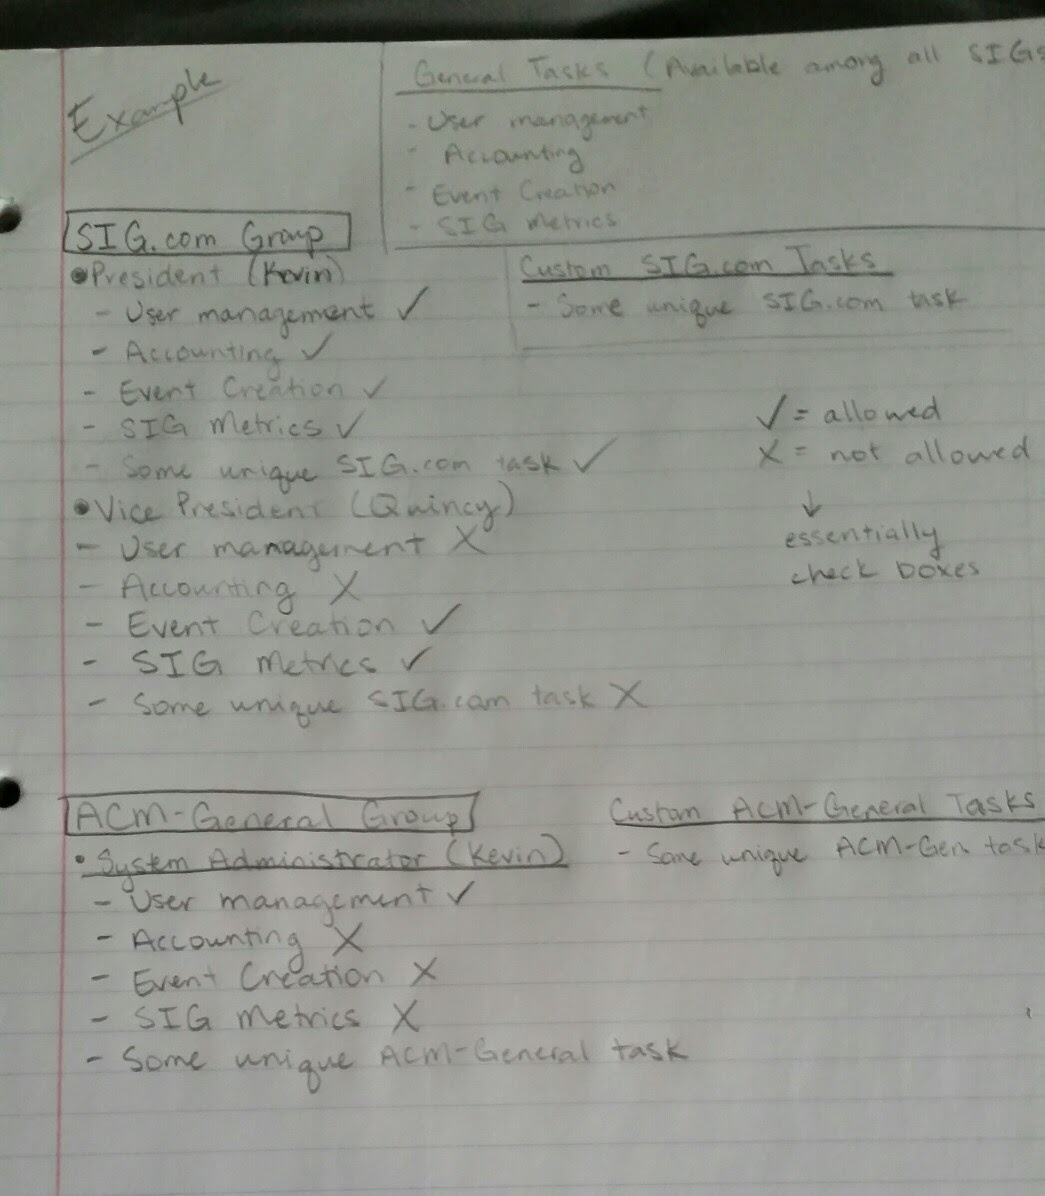
\includegraphics[width=\textwidth,height=\textheight,keepaspectratio]{figures/permissions.jpg}

\subsubsection{Fine-grained Control}
\label{sub-sec:perm_control}
In order to control each of the different permissions in the roles a representative
GUI would look like: 

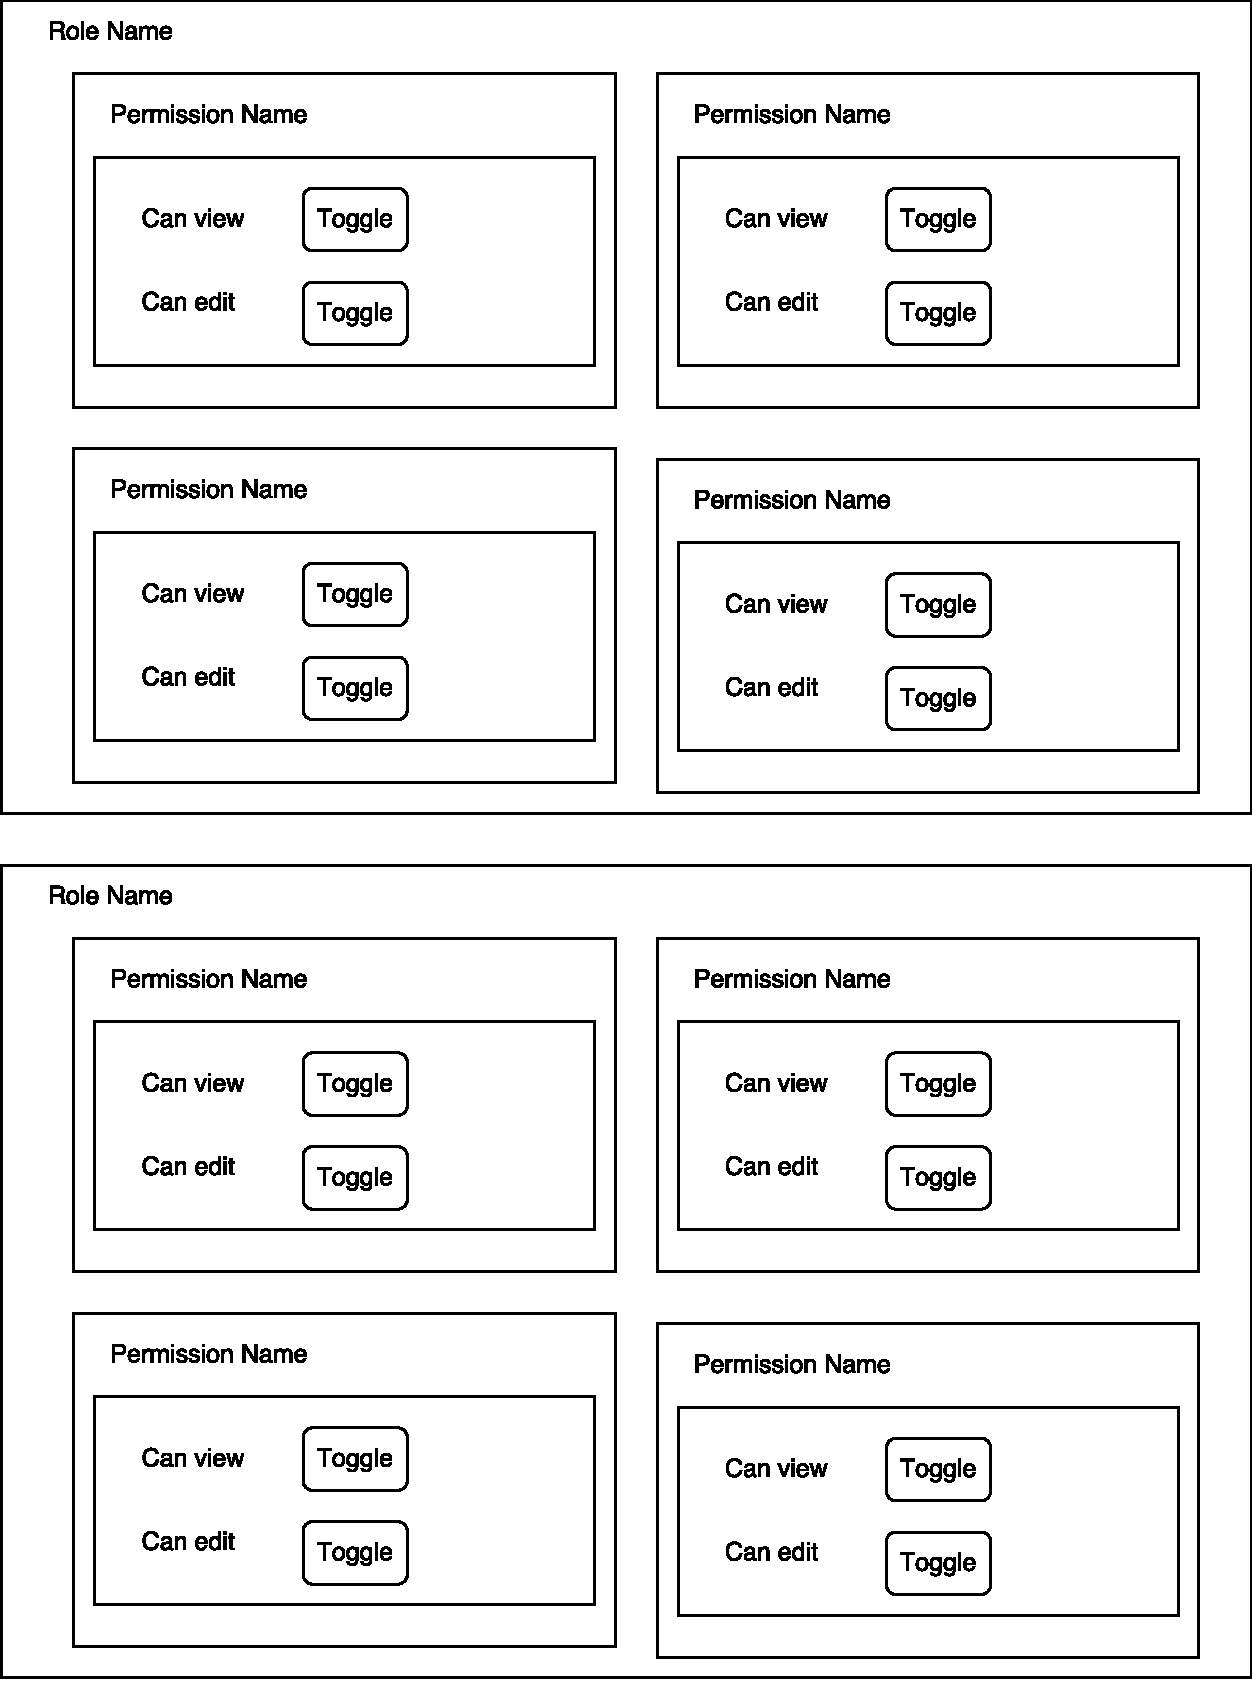
\includegraphics[width=\textwidth,height=\textheight,keepaspectratio]{figures/permissions.pdf}

% TODO: Plan for modular permissions.
\subsubsection{Permissions ideas}
Brainstorming of all permission ideas necessary for the website. Section will be
refined/removed later.
\begin{itemize}
    \item Manage API Keys
    \item Per-model
    \begin{itemize}
        \item GET specific instance
        \item GET all models
        \item DELETE specific instance
        \item Create new instance
        \item Modify existing instance
    \end{itemize}

    \item Per-SIG
    \begin{itemize}
        \item Manage SIG roles / permissions
        \item Create SIG events
        \item Manage SIG members
        \item Manage SIG budget?
    \end{itemize}

    \item Per-view (need to have a better way of modulating this)
    \begin{itemize}
        \item Can GET
        \item Can POST
    \end{itemize}


\end{itemize}
\subsection{Testing}
Testing will be required for every user who wishes to contribute to the code base.
Every developer will be responsible for thoroughly testing their features using Django's
unit-testing framework. Test-driven development is encouraged. 

Before every release, the website will be examined to make sure no visual bug,
cross-browser compatibility, and any other hard-to-test features are allowed
to be released. 

\section{Workflow}
\subsection{Git}
The git workflow the development will be following is located on 
\url{http://nvie.com/posts/a-successful-git-branching-model/}. I recommend
reading the article for a thorough understanding of how it will all piece together.
The part that most developers will need to be concerned about is how to properly
branch and push to the proper place. 

Whenever a developer wants to add a new feature,
the developer will create a branch with the schema \texttt{feature/<feature-name>}. The 
developer will write all the code to establish this feature on that branch. After
the developer has completed the feature, written the necessary documentation, and
properly tested it implementing unit-tests, the developer will then push this
feature to the \texttt{develop} branch for integration testing with all currently
produced features. 

\subsection{Features}
For any feature a developer wishes to add, a GitHub issue must be made detailing
the new feature with a description, a reason why the feature should be added, and
the details of how the feature will be implemented. Even if the developer does
not wish to implement the feature themselves, the issue must be made to allow for
group discussion as well as possible implementation by someone else.

\subsection{Release Cycle}:
Each release cycle will last approximately five weeks. The first week, issues will
be selected from GitHub and added to a GitHub milestone representing all the 
features which will finished before the release. Week 2 and 3 will be used to 
develop these features. During week 4, the feature will be tested and the 
documentation will be checked for readability and accuracy. Week 5 will be an
extra week just in case things get pushed back or a step took longer than
anticipated.


\section{Milestones / Deadlines}
The release cycle up to the 2018 Semester:
\\
\textbf{Release 0.5.0 - 2017.06.30 - 2017.08.25}
\begin{itemize}
    \item Permissions
    \item Event Creation
    \item ACM Membership
\end{itemize}
\textbf{Release 0.6.0: 2017.08.25 - 2017.09.29}
\begin{itemize}
    \item Sponsorship - Why Sponsor Us? and Online Sponsorship Payment
    \item Documentation updated to current state
\end{itemize}
\textbf{Release 0.7.0: 2017.09.29 - 2017.11.03}
\begin{itemize}
    \item Event Management and Event Participation 
\end{itemize}
\textbf{Release 1.0.0: 2017.11.03 - 2017.12.31}
\begin{itemize}
    \item SIG homepage 
    \item User homepage
\end{itemize}

\end{document}
